\documentclass{article}
\usepackage[margin=1in]{geometry}
\usepackage{amsmath, amssymb, amsfonts, enumitem, fancyhdr, tikz}
% get rid of paragraph indent
\setlength{\parindent}{0 pt}
% allow section.equation numbering
\numberwithin{equation}{section}
\usepackage{hyperref}
% make the link colors blue, as well as cite colors. urls are magenta
\hypersetup{colorlinks, linkcolor=blue, citecolor=blue, urlcolor=magenta}

\title{Statistical Learning with Sparsity \\ \Large Worked Exercises}
\author{Derek Huang\thanks{SMBC Capital Markets, Quantitative Strategists.}}
\date{April 4, 2022}

\begin{document}

\newcommand{\newtocsubsection}[1]{%
    \subsection*{#1} \addcontentsline{toc}{subsection}{#1}%
}

\maketitle

%\newpage

\tableofcontents

\newpage

\section{Introduction}

During my time as an undergraduate student at NYU, there was a period where
I found it interesting how the theory of convex optimization was applied by
the field of supervised learning to fit models. One of the topics I was
interested in was sparse optimization, mostly the kinds where sparsity was
enforced by a convex norm constraint, ex. $ \ell^1 $ norm for vectors,
nuclear norm for matrices.

\medskip

To satisfy my interests, I ended up purchasing Hastie, Tibshirani, and
Wainwright's \textit{%
    Statistical Learning with Sparsity: The Lasso and Generalizations%
}, seeing that it was a monograph on the topic. Despite enjoying the portions
of the book that I found time to read, I did not do any of the exercises,
as I didn't properly set aside enough time to attempt them and was a bit fearful that if I couldn't do the exercises, it would somehow prove that my own intelligence was sorely lacking. I no longer feel the same way.

\medskip

Regardless, the worked exercises in this document exist to be a testament
to my own efforts towards understanding and will hopefully be a resource to
anyone else who may be attempting these exercises.

\medskip

\fbox{%
    \parbox{\textwidth}{%
        \textbf{Disclaimer:} This is \textcolor{red}{\textbf{not}} an official
        solution guide for the text. I \textbf{strongly} \textbf{recommend}
        that one attempt the text's exercises \textbf{on} \textbf{their}
        \textbf{own} before consulting this document, as I believe active
        self-learning truly plays an outsized role in determining the depth of
        one's understanding. One's instructors are there to guide and support,
        but all must walk their paths to understanding themselves.%
    }%
}

\section{The Lasso for Linear Models}

\newtocsubsection{Exercise 2.1} \label{sec:2.1}

Let $ \mathbf{x}_j  \in \mathbb{R}^N $ denote the $ j $-th column of the
predictor matrix $ \mathbf{X} \in \mathbb{R}^{N \times d} $, and let
$ \mathbf{y} \in \mathbb{R}^N $ denote the response vector as usual. Under
the assumptions of section 2.4, we have $ \frac{1}{N}\mathbf{1}^\top
\mathbf{y} = 0 $, $ \frac{1}{N}\mathbf{1}^\top\mathbf{x}_j = 0 $,
$ \frac{1}{N}\mathbf{x}_j^\top\mathbf{x}_j = 1 $\footnote{
    In words, the predictors are standardized to zero mean and unit variance,
    while the response is standardized to zero mean.
}.

\medskip

The lasso problem, as introduced in the book, can be written as
\begin{equation} \label{eq:std_lasso}
    \min_\mathbf{w}\frac{1}{2N}\Vert\mathbf{y} - \mathbf{Xw}\Vert_2^2 +
    \lambda\Vert\mathbf{w}\Vert_1
\end{equation}

Let us replace $ \lambda \in (0, \infty) $ with $ \lambda_j \in
(0, \infty) $, where $ \forall j \in \{1, \ldots d\} $, $ \lambda_j
\Rightarrow w_{j'} \in \{1, \ldots d\}, j' \ne j, w_{j'} = 0 $.
With $ \lambda \triangleq \lambda_j $, only $ w_j $ may be nonzero, and
so in that case we can rewrite (\ref{eq:std_lasso}) where
$ \lambda \triangleq \lambda_j $ as
\begin{equation*}
    \min_{w_j}\frac{1}{2N}\sum_{k = 1}^N(y_k - x_{kj}w_j)^2 +
    \lambda_j|w_j|
\end{equation*}

Taking the subderivative of the above expression at its minimizer
$ \hat{w}_j $, we have
\begin{equation*}
    0 \in \left\{
        -\frac{1}{N}\sum_{k = 1}^Nx_{kj}(y_k - x_{kj}\hat{w}_j)
    \right\} +
    \lambda_j\partial|\hat{w}_j| =
    \left\{-\frac{1}{N}\mathbf{x}_j^\top\mathbf{y} + \hat{w}_j\right\} +
    \lambda_j\partial|\hat{w}_j|
\end{equation*}

Note that $ \hat{w}_j = 0 \Rightarrow \partial|\hat{w}_j| = [-1, 1] $. We
must then have $ \left|\frac{1}{N}\mathbf{x}_j^\top\mathbf{y}\right| \le
\lambda_j \Rightarrow \left|\frac{1}{N}\mathbf{x}_j^\top\mathbf{y}\right| $
is the smallest value of $ \lambda $ that guarantees $ \hat{w}_j = 0 $
conditional on $ \hat{w}_{j'} = 0 $, $ \forall j' \in \{1, \ldots d\} $,
$ j' \ne j $. Therefore, the smallest value of $ \lambda $,
which we denote $ \tilde{\lambda} $, that unconditionally guarantees
$ \hat{\mathbf{w}} = \mathbf{0} $, is such that
\begin{equation*}
    \tilde{\lambda} \triangleq
    \frac{1}{N}\max\big\{
        \big|\mathbf{x}_1^\top\mathbf{y}\big|, \ldots
        \big|\mathbf{x}_d^\top\mathbf{y}\big|
    \big\}
\end{equation*}

\newtocsubsection{Exercise 2.2}

The scalar soft-thresholding operator $ \mathcal{S}_\lambda $ presented in
section 2.4.1 is defined such that for $ \lambda \in (0, \infty) $,
\begin{equation} \label{eq:soft_threshold}
    \mathcal{S}_\lambda(x) \triangleq
    \operatorname{sgn}(x)\max\{0, |x| - \lambda\}
\end{equation}

For a scalar predictor, where we have an input vector $ \mathbf{x} \in
\mathbb{R}^N $, the lasso problem (\ref{eq:std_lasso}) simplifies to
\begin{equation} \label{eq:single_lasso}
    \min_w\frac{1}{2N}\sum_{k = 1}^N(y_k - x_kw)^2 + \lambda|w|
\end{equation}

We could solve for the minimizer $ \hat{w} \in \mathbb{R} $ of
(\ref{eq:single_lasso}) by taking a subderivative, but we are explicitly
told not to, so we instead proceed by considering the different cases of
$ \hat{w} $. Naturally, for simplicity, we first suppose that
$ \hat{w} \in (0, \infty) $. In that case, we can take a derivative of
(\ref{eq:single_lasso}) at $ \hat{w} $, and thus have
\begin{equation*}
    0 = -\frac{1}{N}\sum_{k = 1}^Nx_k(y_k - x_k\hat{w}) + \lambda =
    -\frac{1}{N}\mathbf{x}^\top\mathbf{y} + \hat{w} + \lambda \Leftrightarrow
    \hat{w} = \frac{1}{N}\mathbf{x}^\top\mathbf{y} - \lambda
\end{equation*}

Here we use the fact that as in \nameref{sec:2.1}, the input vector
$ \mathbf{x} $ is given standardized, where $ \frac{1}{N}\mathbf{1}^\top
\mathbf{x} = 0 $, $ \frac{1}{N}\mathbf{x}^\top\mathbf{x} = 1 $, so
$ \frac{1}{N}\sum_{k = 1}^Nx_k^2\hat{w} $ simplifies to $ \hat{w} $. Now,
considering the case when $ \hat{w} \in (-\infty, 0) $, we have
\begin{equation*}
    0 = -\frac{1}{N}\mathbf{x}^\top\mathbf{y} + \hat{w} - \lambda
    \Leftrightarrow \hat{w} = \frac{1}{N}\mathbf{x}^\top\mathbf{y} + \lambda
\end{equation*}

Noting that $ \lambda \in (0, \infty) $, we thus have $ \hat{w} \in
(0, \infty) \Leftrightarrow \frac{1}{N}\mathbf{x}^\top\mathbf{y} > \lambda $,
$ \hat{w} \in (-\infty, 0) \Leftrightarrow \frac{1}{N}\mathbf{x}^\top
\mathbf{y} < -\lambda $, which may be simplified into the condition that
$ \hat{w} \ne 0 \Leftrightarrow \left|\frac{1}{N}\mathbf{x}^\top
\mathbf{y}\right| > \lambda $. Therefore, by \textit{modus tollens} in both
directions, $ \hat{w} = 0 \Leftrightarrow \left|\frac{1}{N}\mathbf{x}^\top
\mathbf{y}\right| \le \lambda $. Furthermore, we can express $ \hat{w} $ in
terms of $ \frac{1}{N}\mathbf{x}^\top\mathbf{y} $ such that
\begin{equation*}
    \hat{w} =
    \operatorname{sgn}\left(\frac{1}{N}\mathbf{x}^\top\mathbf{y}\right)
    \max\left\{
        \left|\frac{1}{N}\mathbf{x}^\top\mathbf{y}\right| - \lambda, 0
    \right\} \triangleq
    \mathcal{S}_\lambda\left(\frac{1}{N}\mathbf{x}^\top\mathbf{y}\right)
\end{equation*}

(\ref{eq:soft_threshold}) therefore yields the solution to
(\ref{eq:single_lasso}) when applied to
$ \frac{1}{N}\mathbf{x}^\top\mathbf{y} $.

\newtocsubsection{Exercise 2.3} \label{sec:2.3}

The subgradient, more precisely subderivative, equation for
(\ref{eq:single_lasso}) at a minimizer $ \hat{w} \in \mathbb{R} $ is
\begin{equation} \label{eq:2.3.1}
    0 \in
    \left\{-\frac{1}{N}\sum_{k = 1}^Nx_k(y_k - x_k\hat{w})\right\} +
    \lambda\partial|\hat{w}| =
    \left\{-\frac{1}{N}\mathbf{x}^\top\mathbf{y} + \hat{w}\right\} +
    \lambda\partial|\hat{w}|
\end{equation}

Here we use the fact that $ \mathbf{x} \in \mathbb{R}^N $ is standardized
with $ \frac{1}{N}\mathbf{1}^\top\mathbf{x} = 0 $,
$ \frac{1}{N}\mathbf{x}^\top\mathbf{x} = 1 $. By the standard theory of
subgradients and considering the cases where $ \hat{w} \in (0, \infty) $,
$ \hat{w} \in(-\infty, 0) $, $ \hat{w} = 0 $, we see that
\begin{equation*}
    \begin{split}
            \hat{w} \in (0, \infty) & \Leftrightarrow
            0 \in \left\{
                -\frac{1}{N}\mathbf{x}^\top\mathbf{y} + \hat{w} + \lambda
            \right\} \Leftrightarrow
            \hat{w} = \frac{1}{N}\mathbf{x}^\top\mathbf{y} - \lambda
            \Leftrightarrow \frac{1}{N}\mathbf{x}^\top\mathbf{y} > \lambda \\
            \hat{w} \in (-\infty, 0) & \Leftrightarrow
            0 \in \left\{
                -\frac{1}{N}\mathbf{x}^\top\mathbf{y} + \hat{w} - \lambda
            \right\} \Leftrightarrow
            \hat{w} = \frac{1}{N}\mathbf{x}^\top\mathbf{y} + \lambda
            \Leftrightarrow \frac{1}{N}\mathbf{x}^\top\mathbf{y} < -\lambda \\
            \hat{w} = 0 & \Leftrightarrow
            0 \in \left\{-\frac{1}{N}\mathbf{x}^\top\mathbf{y}\right\} +
            \lambda[-1, 1] \Leftrightarrow
            \left|-\frac{1}{N}\mathbf{x}^\top\mathbf{y}\right| \le \lambda
    \end{split}
\end{equation*}

We can write our results more neatly in the style of the book as
\begin{equation} \label{eq:2.3.2}
    \hat{w} = \left\{
        \begin{aligned}
            & \frac{1}{N}\mathbf{x}^\top\mathbf{y} - \lambda,
            & & \frac{1}{N}\mathbf{x}^\top\mathbf{y} > \lambda \\
            & 0, &
            & \frac{1}{N}\left|\mathbf{x}^\top\mathbf{y}\right| \le \lambda \\
            & \frac{1}{N}\mathbf{x}^\top\mathbf{y} + \lambda,
            & & \frac{1}{N}\mathbf{x}^\top\mathbf{y} < -\lambda
        \end{aligned}
    \right.
\end{equation}

Finally, from (\ref{eq:soft_threshold}), it's clear that we can express
(\ref{eq:2.3.2}) more succinctly with $ \mathcal{S}_\lambda $ as
\begin{equation} \label{eq:2.3.3}
    \hat{w} =
    \mathcal{S}_\lambda\left(\frac{1}{N}\mathbf{x}^\top\mathbf{y}\right)
\end{equation}

\newtocsubsection{Exercise 2.4}

The subgradient equation for (\ref{eq:std_lasso}) at a minimizer
$ \mathbf{\hat{w}} \in \mathbb{R}^d $ in vector-matrix notation is
\begin{equation*}
    \mathbf{0} \in \left\{
        -\frac{1}{N}\mathbf{X}^\top(\mathbf{y} - \mathbf{X}\hat{\mathbf{w}})
    \right\} +
    \lambda\partial\Vert\hat{\mathbf{w}}\Vert_1
\end{equation*}

We can also write the subderivative equation for each predictor $ j \in
\{1, \ldots d\} $, which is
\begin{equation} \label{eq:2.4.1}
    0 \in \left\{
        -\frac{1}{N}\mathbf{x}_j^\top(\mathbf{y} - \mathbf{X}\hat{\mathbf{w}})
    \right\} +
    \lambda\partial|\hat{w}_j|
\end{equation}

From (\ref{eq:2.4.1}), we can derive the update applied to the $ j $th
coefficient $ w_j \in \mathbb{R} $ at each iteration of coordinate descent
by rewriting in terms of $ w_j $ and inspecting the subderivative equation
as in \nameref{sec:2.3}. First, we note $ \mathbf{X}\mathbf{w} $ can be
written as $ \sum_{j = 1}^dw_j\mathbf{x}_j $, and so letting
$ \tilde{P}_j \triangleq\{1, \ldots d\} \setminus \{j\} $,
$ \mathbf{r}_j \triangleq \mathbf{y} -
\sum_{j' \in \tilde{P}_j}w_{j'}\mathbf{x}_{j'} $, we have
\begin{equation} \label{eq:2.4.2}
    0 \in \left\{
        -\frac{1}{N}\mathbf{x}_j^\top(\mathbf{r}_j - w_j\mathbf{x}_j)
    \right\} +
    \lambda\partial|w_j| =
    \left\{-\frac{1}{N}\mathbf{x}_j^\top\mathbf{r}_j + w_j\right\} +
    \lambda\partial|w_j|
\end{equation}

Here we use the fact that (\ref{eq:std_lasso}) assumes $ \forall j \in
\{1, \ldots d\} $, $ \frac{1}{N}\mathbf{x}_j^\top\mathbf{x}_j = 1 $, i.e.
predictors have unit variance. Now, since (\ref{eq:2.4.2}) is just
(\ref{eq:2.3.1}) with $ \hat{w} $ replaced by $ w_j $ and $ \mathbf{x} $,
$ \mathbf{y} $ replaced with $ \mathbf{x}_j $, $ \mathbf{r}_j $, it follows
that the solution to (\ref{eq:2.4.2}) is (\ref{eq:2.3.3}) with the same
replacements for $ \hat{w} $, $ \mathbf{x} $, $ \mathbf{y} $. Therefore, the
coordinate descent update for $ w_j $ is
\begin{equation} \label{eq:2.4.3}
    w_j \leftarrow \mathcal{S}_\lambda\left(
        \frac{1}{N}\mathbf{x}_j^\top\mathbf{r}_j
    \right)
\end{equation}

We may also write (\ref{eq:2.4.3}) more explicitly in terms of the full
residuals $ \mathbf{r} \triangleq \mathbf{y} - \mathbf{Xw} $. We see that
\begin{equation} \label{eq:2.4.4}
    0 \in \left\{-\frac{1}{N}\mathbf{x}_j^\top\mathbf{r}\right\} +
    \lambda\partial|w_j| =
    \left\{
        -\left(w_j + \frac{1}{N}\mathbf{x}_j^\top\mathbf{r}\right) + w_j
    \right\} +
    \lambda\partial|w_j|
\end{equation}

The parenthetical grouping is intentional, as by comparing (\ref{eq:2.4.4})
against (\ref{eq:2.4.2}), where the latter leads to (\ref{eq:2.4.3}), we know
the $ w_j $ coordinate descent update can be written as
\begin{equation*}
    w_j \leftarrow \mathcal{S}_\lambda\left(
        w_j + \frac{1}{N}\mathbf{x}_j^\top\mathbf{r}
    \right)
\end{equation*}

\newtocsubsection{Exercise 2.7}

Let us consider the [random] response vector $ \mathbf{y} $, where
$ \mathbf{y}(\Omega) = \mathbb{R}^N $. Suppose we model $ \mathbf{y} $
using a non-adaptive linear model with independent, finite variance
additive errors. Then,
\begin{equation} \label{eq:std_linear_model}
    \mathbf{y} \triangleq \mathbf{Xw} + \varepsilon
\end{equation}

Here $ \mathbf{X} $ is the [random] input matrix, assumed
centered\footnote{
    We omit the intercept $ b $, since if the inputs are centered, for
    fixed $ \mathbf{y} $, $ \mathbf{X} $, its estimate $ \hat{b} \triangleq
    \frac{1}{N}\big(\mathbf{1}^\top\mathbf{y} -
    \mathbf{1}^\top\mathbf{X}\hat{\mathbf{w}}\big) $.
}, where $ \mathbf{X}(\Omega) = \mathbb{R}^{N \times d} $, $ \mathbf{w} \in
\mathbb{R}^d $ the true parameter vector, and $ \varepsilon $ the error
vector with i.i.d. components, where $ \forall k \in\{1, \ldots N\} $,
$ \mathbb{E}[\varepsilon_k] = 0 $, $ \operatorname{Var}(\varepsilon_k) =
\sigma^2 $. To fit (\ref{eq:std_linear_model}) by least squares, we want to
solve the convex problem
\begin{equation} \label{eq:std_linear_lsq}
    \min_\mathbf{w}\Vert\mathbf{y} - \mathbf{Xw}\Vert_2^2
\end{equation}

Let us assume that our $ d < N $ predictors are not collinear\footnote{
    If $ \operatorname{rank}(\mathbf{X}) \le \min\{N, d\} $, it is easy to
    see from our solution that the model's degrees of freedom will be
    $ \operatorname{rank}(\mathbf{X}) $.
}, i.e. $ \operatorname{rank}(\mathbf{X}) = d $. To simplify our analysis,
by [compact] singular value decomposition, we can write $ \mathbf{X} =
\mathbf{U\Sigma V}^\top $, where $ \mathbf{U} $, $ \mathbf{V} $ have $ d $
orthonormal columns and $ \mathbf{\Sigma} $ is $ d \times d $ with positive
diagonal. Since the minimizer $ \hat{\mathbf{w}} $ of
(\ref{eq:std_linear_lsq}) is such that $ \mathbf{X}^\top\mathbf{X}
\hat{\mathbf{w}} = \mathbf{X}^\top\mathbf{y} $, then
\begin{equation*}
    \mathbf{X}^\top\mathbf{X}\hat{\mathbf{w}} =
    \mathbf{V\Sigma}^2\mathbf{V}^\top\hat{\mathbf{w}} =
    \mathbf{V\Sigma U}^\top\mathbf{y} \Rightarrow
    \mathbf{V}^\top\hat{\mathbf{w}} =
    \mathbf{\Sigma}^{-1}\mathbf{U}^\top\mathbf{y}
\end{equation*}

Since the [random] predicted values $ \hat{\mathbf{y}} $ are such that
$ \hat{\mathbf{y}} \triangleq \mathbf{X}\hat{\mathbf{w}} $, we can use the
above result to write $ \hat{\mathbf{y}} $ in terms of $ \varepsilon $,
since with $ \mathbf{X} $ fixed $ \varepsilon $ becomes the only source of
randomness. We therefore see that
\begin{equation} \label{eq:2.7.1}
    \hat{\mathbf{y}} =
    \mathbf{U\Sigma}\big(\mathbf{V}^\top\hat{\mathbf{w}}\big) =
    \mathbf{UU}^\top\big(
        \mathbf{U\Sigma V}^\top\mathbf{w} + \varepsilon
    \big) = \mathbf{Xw} + \mathbf{UU}^\top\varepsilon
\end{equation}

As given in the text, the degrees of freedom $ \operatorname{df}(
\hat{\mathbf{y}}) $ of the specified linear model is such that
\begin{equation*}
    \operatorname{df}(\hat{\mathbf{y}}) \triangleq
    \frac{1}{\sigma^2}\sum_{k = 1}^N
    \operatorname{cov}(\hat{y}_k, y_k \mid \mathbf{X})
\end{equation*}

Since $ \operatorname{cov}(\hat{y}_k, y_k \mid \mathbf{X}) =
\mathbb{E}[\hat{y}_ky_k \mid \mathbf{X}] -
\mathbb{E}[\hat{y}_k \mid \mathbf{X}]\mathbb{E}[y_k \mid \mathbf{X}] $, by
linearity of expectation and by (\ref{eq:2.7.1}) we have
\begin{equation} \label{eq:2.7.2}
    \operatorname{df}(\hat{\mathbf{y}}) =
    \frac{1}{\sigma^2}
    \mathbb{E}\big[\hat{\mathbf{y}}^\top\mathbf{y} \ \big| \ \mathbf{X}\big] -
	\frac{1}{\sigma^2}\mathbb{E}[\hat{\mathbf{y}} \mid \mathbf{X}]^\top
    \mathbb{E}[\mathbf{y} \mid \mathbf{X}]
\end{equation}

Expanding the first and second terms of (\ref{eq:2.7.2}) and noting
$ \mathbb{E}[\varepsilon \mid \mathbf{X}] = \mathbf{0} $, we have from
(\ref{eq:std_linear_model}) and (\ref{eq:2.7.1})
\begin{equation*}
    \begin{split}
        \mathbb{E}\big[
            \hat{\mathbf{y}}^\top\mathbf{y} \ \big| \ \mathbf{X}
        \big] & =
        \mathbf{w}^\top\mathbf{X}^\top\mathbf{Xw} +
        \mathbf{w}^\top\mathbf{X}^\top
        \mathbb{E}[\varepsilon \mid \mathbf{X}] +
        \mathbb{E}[\varepsilon \mid \mathbf{X}]^\top
        \mathbf{UU}^\top\mathbf{Xw} +
        \mathbb{E}\big[
            \varepsilon^\top\mathbf{UU}^\top\varepsilon \ \big| \
            \mathbf{X}
        \big] \\ & =
        \mathbf{w}^\top\mathbf{X}^\top\mathbf{Xw} +
        \mathbb{E}\big[
            \varepsilon^\top\mathbf{UU}^\top\varepsilon \ \big| \
            \mathbf{X}
        \big] \\
        \mathbb{E}[\hat{\mathbf{y}} \mid \mathbf{X}]^\top
        \mathbb{E}[\mathbf{y} \mid \mathbf{X}] & =
        \mathbf{w}^\top\mathbf{X}^\top\mathbf{Xw}
    \end{split}
\end{equation*}

We thus see that $ \operatorname{df}(\hat{\mathbf{y}}) = \frac{1}{\sigma^2}
\mathbb{E}\big[\varepsilon^\top\mathbf{UU}^\top\varepsilon \ \big| \
\mathbf{X}\big] $. Letting $ \mathbf{u}_j $ denote the $ j $th column of
$ \mathbf{U} $, then
\begin{equation*}
    \operatorname{df}(\hat{\mathbf{y}}) =
    \frac{1}{\sigma^2}\mathbb{E}\left[
        \begin{bmatrix}
            \ \varepsilon^\top\mathbf{u}_1 &
            \ldots &
            \varepsilon^\top\mathbf{u}_d \
        \end{bmatrix}
        \begin{bmatrix}
            \ \mathbf{u}_1^\top\varepsilon \ \\
            \ \vdots \ \\
            \ \mathbf{u}_d^\top\varepsilon \
        \end{bmatrix}
        \ \middle\vert \ \mathbf{X}
    \right] =
    \frac{1}{\sigma^2}\mathbb{E}\left[
        \sum_{j = 1}^d\big(\mathbf{u}_j^\top\varepsilon\big)^2
        \ \middle\vert \ \mathbf{X}
    \right] =
    \frac{1}{\sigma^2}\sum_{j = 1}^d\mathbb{E}\left[
        \big(\mathbf{u}_j^\top\varepsilon\big)^2
        \ \middle\vert \ \mathbf{X}
    \right]
\end{equation*}

Since $ \mathbb{E}\big[\mathbf{u}_j^\top\varepsilon \ \big| \
\mathbf{X}\big] = 0 $, then $ \mathbb{E}\left[\big(\mathbf{u}_j^\top
\varepsilon\big)^2 \ \middle\vert \ \mathbf{X}\right] = \operatorname{Var}
\big(\mathbf{u}_j^\top\varepsilon \ \big| \ \mathbf{X}\big) $. Recalling
that each $ \varepsilon_1, \ldots \varepsilon_N $ is i.i.d. with
$ \mathbb{E}[\varepsilon_k] = 0 $, $ \operatorname{Var}(\varepsilon_k) =
\sigma^2 $, $ \varepsilon \perp \mathbf{X} $, we see that
$ \operatorname{Var}\big(\mathbf{u}_j^\top\varepsilon \ \big| \
\mathbf{X}\big) = \sum_{k = 1}^Nu_{jk}^2\operatorname{Var}(\varepsilon_k) =
\sigma^2\mathbf{u}_j^\top\mathbf{u}_j = \sigma^2 $. Note that
$ \mathbf{u}_j^\top\mathbf{u}_j = 1 $ by the definition of the orthonormal
vector. Therefore, we see that
\begin{equation*}
    \operatorname{df}(\hat{\mathbf{y}}) =
    \frac{1}{\sigma^2}\sum_{j = 1}^d\operatorname{Var}\big(
        \mathbf{u}_j^\top\varepsilon \ \big| \ \mathbf{X}
    \big) = d
\end{equation*}

Therefore, a linear model fit by least squares using $ d $ non-collinear
predictors has exactly $ d $ degrees of freedom.

\newtocsubsection{Exercise 2.10}

We consider a robust version of least-squares linear regression, i.e. the
min-max constrained problem
\begin{equation} \label{eq:robust_linear_lsq}
    \begin{array}{rl}
        % note: prefer \boldsymbol over \pmb for bold styling that is more
        % consistent with the default \mathbf style
        \displaystyle\min_\mathbf{w}\max_{\boldsymbol{\Delta}} &
        \frac{1}{2N}\Vert\mathbf{y} -
        (\mathbf{X} + \boldsymbol{\Delta})\mathbf{w}\Vert_2^2 \\
        \text{s.t.} & \boldsymbol{\Delta} \in \mathcal{U}_\mathbf{c}
    \end{array}
\end{equation}

Here $ \mathbf{y} \in \mathbb{R}^N $, $ \mathbf{X}, \boldsymbol{\Delta} \in
\mathbb{R}^{N \times d} $, $ \mathbf{c}, \mathbf{w} \in \mathbb{R}^d $, and
$
    \mathcal{U}_\mathbf{c} \triangleq \left\{
        \begin{bmatrix}
             \ \boldsymbol{\delta}_1 & \ldots & \boldsymbol{\delta}_d \
        \end{bmatrix} \in
        \mathbb{R}^{N \times d} : \Vert\boldsymbol{\delta}_k\Vert_2 \le c_k,
        \forall k \in \{1, \ldots d\}
    \right\}
$%
, where $ \mathbf{c} \succeq \mathbf{0} $. Furthermore,
$ \frac{1}{N}\mathbf{1}^\top\mathbf{X} = \mathbf{0} $,
$ \frac{1}{N}\mathbf{1}^\top\mathbf{y} = 0 $,
$ \frac{1}{N}\mathbf{X}^\top\mathbf{X} $ a correlation matrix. Considering
the inner problem, we can expand and drop terms without
$ \boldsymbol{\Delta} $ to get
\begin{equation*}
    \begin{array}{rl}
        \displaystyle\max_{\boldsymbol{\Delta}} &
        -2\mathbf{y}^\top\boldsymbol{\Delta}\mathbf{w} +
        2\mathbf{w}^\top\mathbf{X}^\top\boldsymbol{\Delta}\mathbf{w} +
        \mathbf{w}^\top\boldsymbol{\Delta}^\top\boldsymbol{\Delta}\mathbf{w} \\
        \text{s.t.} & \boldsymbol{\Delta} \in \mathcal{U}_\mathbf{c}
    \end{array}
\end{equation*}

To better organize the terms containing $ \boldsymbol{\Delta} $, we can
rewrite the above as
\begin{equation} \label{eq:2.10.1}
    \begin{array}{rl}
        \displaystyle\max_{\boldsymbol{\Delta}} &
        \Vert\boldsymbol{\Delta}\mathbf{w}\Vert_2^2 -
        2(\mathbf{y} - \mathbf{Xw})^\top\boldsymbol{\Delta}\mathbf{w} \\
        \text{s.t.} & \boldsymbol{\Delta} \in \mathcal{U}_\mathbf{c}
    \end{array}
\end{equation}

Denoting the matrix derivative of the objective in (\ref{eq:2.10.1}) as
$ \nabla g_\mathbf{w} $, we see that
\begin{equation} \label{eq:2.10.2}
    \nabla g_\mathbf{w}(\boldsymbol{\Delta}) \propto
    \boldsymbol{\Delta}\mathbf{ww}^\top -
    (\mathbf{y} - \mathbf{Xw})\mathbf{w}^\top
\end{equation}

Since (\ref{eq:2.10.1}) has a convex objective, a maximizer
$ \hat{\boldsymbol{\Delta}} \in \mathcal{U}_\mathbf{c} $ must also be a
maximizer for $ \max_{\boldsymbol{\Delta} \in
\mathcal{U}_\mathbf{c}}\nabla g_\mathbf{w}(\boldsymbol{\Delta}) $, where
naturally $ \hat{\boldsymbol{\Delta}} $ is on the boundary of
$ \mathcal{U}_\mathbf{c} $. Since in (\ref{eq:2.10.1}), (\ref{eq:2.10.2})
$ \boldsymbol{\Delta} $ is always multiplied by $ \mathbf{w} $, one choice is
to define $ \hat{\boldsymbol{\Delta}} $ as a rank-1 matrix with rows parallel
to $ \mathbf{w} $. Written more explicitly,
\begin{equation} \label{eq:2.10.3}
    \hat{\boldsymbol{\Delta}} \triangleq N^{-1 / 2}\mathbf{1}_N\begin{bmatrix}
        \ c_1\operatorname{sgn}(w_1) & \ldots & c_d\operatorname{sgn}(w_d) \
    \end{bmatrix}
\end{equation}

We can equivalently express (\ref{eq:2.10.3}) in terms of
$ \hat{\boldsymbol{\delta}}_k $, where $ \forall k \in \{1, \ldots d\} $,
\begin{equation} \label{eq:2.10.4}
    \hat{\boldsymbol{\delta}}_k \triangleq
    \frac{c_k}{\sqrt{N}}{\operatorname{sgn}(w_k)}\mathbf{1}_N
\end{equation}

It is clear from (\ref{eq:2.10.4}) that
$ \Vert\hat{\boldsymbol{\delta}}_k\Vert_2 \le c_k $, where the inequality is
tight if $ \mathbf{w} $ has no zeros. Furthermore, defining a weighted
$ \ell^1 $ norm as $ \Vert\mathbf{w}\Vert_{1, \mathbf{c}} \triangleq
\sum_{k = 1}^dc_k|w_k| $, $ \mathbf{c} \succeq \mathbf{0} $, we see that
\begin{equation} \label{eq:2.10.5}
    \hat{\Delta}\mathbf{w} =
    N^{-1 / 2}\left(\sum_{k = 1}^dc_k|w_k|\right)\mathbf{1}_N \triangleq
    N^{-1 / 2}\Vert\mathbf{w}\Vert_{1, \mathbf{c}}\mathbf{1}_N
\end{equation}

From (\ref{eq:2.10.5}), we can therefore write (\ref{eq:robust_linear_lsq}) as
the convex unconstrained minimization problem
\begin{equation} \label{eq:2.10.6}
    \begin{array}{rl}
        \displaystyle\min_\mathbf{w} &
        \frac{1}{2N}\left\Vert
            \mathbf{y} - \mathbf{Xw} -
            \frac{1}{\sqrt{N}}\Vert\mathbf{w}\Vert_{1, \mathbf{c}}\mathbf{1}_N
        \right\Vert_2^2
    \end{array}
\end{equation}

However, direct analysis of the above would be quite difficult. Fortunately,
recalling the standardization assumptions made on $ \mathbf{y} $,
$ \mathbf{X} $, we can do some simplification and thus see that
\begin{equation*}
    \begin{split}
        \left\Vert
            \mathbf{y} - \mathbf{Xw} -
            \frac{1}{\sqrt{N}}\Vert\mathbf{w}\Vert_{1, \mathbf{c}}\mathbf{1}_N
        \right\Vert_2^2 & =
        \left(
            \mathbf{y}^\top\mathbf{y} - 2\mathbf{y}^\top\mathbf{Xw} +
            \mathbf{w}^\top\mathbf{X}^\top\mathbf{Xw}
        \right) -
        \frac{1}{\sqrt{N}}\Vert\mathbf{w}\Vert_{1, \mathbf{c}}
        \mathbf{1}_N^\top(\mathbf{y} - \mathbf{Xw}) +
        \Vert\mathbf{w}\Vert_{1, \mathbf{c}}^2 \\
        & =
        \Vert\mathbf{y} - \mathbf{Xw}\Vert_2^2 +
        \Vert\mathbf{w}\Vert_{1, \mathbf{c}}^2
    \end{split}
\end{equation*}

Therefore, instead of (\ref{eq:2.10.6}), we can consider the less threatening
yet equivalent problem
\begin{equation} \label{eq:2.10.7}
    \begin{array}{rl}
        \displaystyle\min_\mathbf{w} &
        \Vert\mathbf{y} - \mathbf{Xw}\Vert_2^2 +
        \Vert\mathbf{w}\Vert_{1, \mathbf{c}}^2
    \end{array}
\end{equation}

Note that for some $ \kappa \in (0, \infty) $, (\ref{eq:2.10.7}) is equivalent
to the Lagrangian for
\begin{equation} \label{eq:2.10.8}
    \begin{array}{rl}
        \displaystyle\min_\mathbf{w} &
        \Vert\mathbf{w}\Vert_{1, \mathbf{c}}^2 \\
        \text{s.t} &
        \frac{1}{2N}\Vert\mathbf{y} - \mathbf{Xw}\Vert_2^2 \le \kappa
    \end{array}
\end{equation}

Here $ \mathbf{c} $ has been redefined with the scale factor $ \frac{1}{2N} $.
Changes in the Lagrange multiplier used in the Lagrangian of (\ref{eq:2.10.8})
can be reflected in the same way, i.e. if the Lagrange multiplier is increased,
we can scale $ \mathbf{c} $ down by some $ \varepsilon \in (0, 1) $. Also, for
any $ \hat{\mathbf{w}} $ that satisfies (\ref{eq:2.10.8}), $ \hat{\mathbf{w}} $
necessarily satisfies
\begin{equation} \label{eq:2.10.9}
    \begin{array}{rl}
        \displaystyle\min_\mathbf{w} & \Vert\mathbf{w}\Vert_{1, \mathbf{c}} \\
        \text{s.t} &
        \frac{1}{2N}\Vert\mathbf{y} - \mathbf{Xw}\Vert_2^2 \le \kappa
    \end{array}
\end{equation}

Writing (\ref{eq:2.10.9}) in its Lagrangian form, where again $ \mathbf{c} $
can be rescaled as necessary to reflect the magnitude of the Lagrange
multiplier, we have our desired result, i.e. solving
(\ref{eq:robust_linear_lsq}) is equivalent to solving
\begin{equation}
    \begin{array}{rl}
        \displaystyle\min_\mathbf{w} &
        \frac{1}{2N}\Vert\mathbf{y} - \mathbf{Xw}\Vert_2^2 +
        \Vert\mathbf{w}\Vert_{1, \mathbf{c}}
    \end{array}
\end{equation}

\section{Generalized Linear Models}

\newtocsubsection{Exercise 3.1}

\fbox{%
    \parbox{\textwidth}{%
        \textbf{Note:} I believe the authors made a semantic error in the
        problem's wording, as it should be the parameter estimates that
        are, or rather tend towards being, infinite, not the likelihood
        estimates themselves, as those are constrained within $ (0, 1) $
        given any $ \mathbf{w} \in \mathbb{R}^d $. Also, to be more precise,
        the optimal value of the unregularized objective is reached only in
        the limit, and is never achieved by any finite $ \mathbf{w} $.
    }%
}

\medskip

Consider training data pairs $ \mathcal{D} \triangleq
\{(\mathbf{x}_1, y_1), \ldots (\mathbf{x}_N, y_N)\} $, where $ \forall k \in
\{1, \ldots N\} $, $ \mathbf{x}_k \in \mathbb{R}^d $, $ y_k \in \{-1, 1\} $.
We choose the symmetric labeling scheme without loss of generality for a more
elegant analysis. Since the two labeled classes of points are linearly
separable, $ \exists \tilde{\mathbf{w}} \in \mathbb{R}^d $,
$ \tilde{b} \in \mathbb{R} $, $ \tilde{f}(\mathbf{x}) \triangleq
\tilde{\mathbf{w}}^\top\mathbf{x} + \tilde{b} $ s.t.
$ \forall (\mathbf{x}, y) \in \mathcal{D} $, $ y\tilde{f}(\mathbf{x}) > 0
\Rightarrow y = \operatorname{sgn} \circ \tilde{f}(\mathbf{x}) $. In words,
margin always positive $ \Rightarrow \tilde{f} $ perfectly classifies
each data point.

\medskip

Under the $ \{-1, 1\} $ labeling scheme, the [scaled] negative log-likelihood
for two-class logistic regression is
\begin{equation} \label{eq:logreg_binary_mle}
    \min_{\mathbf{w}, b}\frac{1}{N}\sum_{k = 1}^N\log\left(
        1 + e^{-y_k\left(\mathbf{w}^\top\mathbf{x}_k + b\right)}
    \right)
\end{equation}

Consider some $ \varepsilon \in (0, \infty) $. Since
$ \forall (\mathbf{x}, y) \in \mathcal{D} $, $ y\tilde{f}(\mathbf{x}) > 0 $,
obviously $ \varepsilon y\tilde{f}(\mathbf{x}) > 0 \Rightarrow
\varepsilon\tilde{\mathbf{w}}, \varepsilon\tilde{b} $ also results in perfect
linear separability of the two classes. However, note that
\begin{equation*}
    \lim_{\varepsilon \rightarrow \infty}\frac{1}{N}\sum_{k = 1}^N\log\left(
        1 + e^{-\varepsilon y_k\tilde{f}(\mathbf{x}_k)}
    \right) =
    \frac{1}{N}\sum_{k = 1}^N\log\left(
        1 + \lim_{\varepsilon \rightarrow \infty}
        e^{-\varepsilon y_k\tilde{f}(\mathbf{x}_k)}
    \right) =
    \log 1 = 0
\end{equation*}

Here we use the fact that continuous functions respect limits and that
$ \forall a \in (0, \infty) $,
$ \lim_{\varepsilon \rightarrow \infty}e^{-a\varepsilon} = 0 $. Clearly,
(\ref{eq:logreg_binary_mle}) approaches its optimal value of zero in the
limit as the norms of positive multiples of $ \tilde{\mathbf{w}} $,
$ \tilde{b} $ approach infinity. Furthermore, we can show that the fitted
probabilities $ \tilde{\mathbb{P}}_\varepsilon\{Y = 1 \mid X = \mathbf{x}\} $,
$ \tilde{\mathbb{P}}_\varepsilon\{Y = -1 \mid X = \mathbf{x}\} $ are
well-defined. Let $ \tilde{\mathbb{P}}_\varepsilon
\{Y = y \mid X = \mathbf{x}\} $ be defined such that
\begin{equation} \label{eq:3.1.1}
    \tilde{\mathbb{P}}_\varepsilon\{Y = y \mid X = \mathbf{x}\} \triangleq
    \frac{1}{1 + e^{-\varepsilon y\tilde{f}(\mathbf{x})}} \triangleq
    \sigma\circ\varepsilon y\tilde{f}(\mathbf{x})
\end{equation}

Here $ \sigma : \mathbb{R} \rightarrow (0, 1) $ is the sigmoid function,
defined such that $ \sigma(z) \triangleq \frac{1}{1 + e^{-z}} $. Note that
(\ref{eq:3.1.1}) results from simple rearrangement of the standard linear
model for the log of the likelihood ratio, i.e.
\begin{equation*}
    \log\frac{
        \tilde{\mathbb{P}}_\varepsilon\{Y = 1 \mid X = \mathbf{x}\}
    }{
        \tilde{\mathbb{P}}_\varepsilon\{Y = -1 \mid X = \mathbf{x}\}
    } =
    \varepsilon\tilde{f}(\mathbf{x})
\end{equation*}

We note that after solving for $ \tilde{\mathbb{P}}_\varepsilon
\{Y = 1 \mid X = \mathbf{x}\} $, we can see that
\begin{equation*}
    \begin{split}
        \tilde{\mathbb{P}}_\varepsilon\{Y = 1 \mid X = \mathbf{x}\} & =
        \frac{
            e^{\varepsilon\tilde{f}(\mathbf{x})}
        }{
            1 + e^{\varepsilon\tilde{f}(\mathbf{x})}
        } =
        \frac{1}{1 + e^{-\varepsilon\tilde{f}(\mathbf{x})}} \triangleq
        \sigma\circ\varepsilon\tilde{f}(\mathbf{x}) \\
        \tilde{\mathbb{P}}_\varepsilon\{Y = -1 \mid X = \mathbf{x}\} & =
        1 - \tilde{\mathbb{P}}_\varepsilon\{Y = 1 \mid X = \mathbf{x}\} =
        \frac{1}{1 + e^{\varepsilon\tilde{f}(\mathbf{x})}} \triangleq
        \sigma\circ -\varepsilon\tilde{f}(\mathbf{x})
    \end{split}
\end{equation*}

For fixed $ y \in \{-1, 1\} $ and $ \forall \varepsilon \in (0, \infty) $,
$ \tilde{\mathbb{P}}_\varepsilon\{Y = y \mid X = \mathbf{x}\} $ as defined
in (\ref{eq:3.1.1}) is a well-defined function of $ \mathbf{x} $, as it is
just a composition of a bijective\footnote{
    $ \exists\sigma^{-1} : (0, 1) \rightarrow \mathbb{R} $ where
    $ \sigma^{-1}(z) \triangleq -\log\left(z^{-1} - 1\right) $.
}, strictly monotone increasing\footnote{
    $ \exists\sigma': \mathbb{R} \rightarrow (0, 1) $ where
    $ \sigma'(z) \triangleq \frac{e^{-z}}{(1 + e^{-z})^2} =
    \frac{1}{1 + e^{-z}}\left(\frac{e^{-z}}{1 + e^{-z}}\right) \triangleq
    \sigma(z)(1 - \sigma(z)) $. Note $ (-\infty, 0] \cap
    \operatorname{im}\sigma' = \emptyset $.
}
function with an affine function. Clearly, $ \operatorname{dom}\varepsilon
y\tilde{f} = \mathbb{R}^d $, $ \operatorname{im}\varepsilon
y\tilde{f} \subseteq \mathbb{R} $, so $ \sigma\circ\varepsilon y\tilde{f} $
is itself well-defined as a function. It is also clear that from inspecting
(\ref{eq:3.1.1}) that $ \lim_{\varepsilon \rightarrow \infty}
\tilde{\mathbb{P}}_\varepsilon\{Y = y \mid X = \mathbf{x}\} =
\mathbb{I}_{(0, \infty)}\circ y\tilde{f}(\mathbf{x}) $, i.e. a step function
of the margin.

\newtocsubsection{Exercise 3.2}

Consider an input point and label pair $ (\mathbf{x}, y) \in \mathbb{R}^d
\times \{-1, 1\} $, a linear classification function
$ f : \mathbb{R}^d \rightarrow \mathbb{R} $ where
$ f(\mathbf{x}) \triangleq \mathbf{w}^\top\mathbf{x} + b $, and its
corresponding decision boundary $ \mathcal{B} \triangleq \{\mathbf{x}' \in
\mathbb{R}^d : f(\mathbf{x}') = 0\} $. Note that $ \forall \mathbf{x}',
\tilde{\mathbf{x}} \in \mathcal{B} $, $ f(\mathbf{x}') -
f(\tilde{\mathbf{x}}) = \mathbf{w}^\top(\mathbf{x}' - \tilde{\mathbf{x}}) =
0 \Rightarrow \mathbf{w} \perp \mathbf{x}' - \tilde{\mathbf{x}} $, i.e.
$ \mathbf{w} $, and thus $ \mathbf{w} / \Vert\mathbf{w}\Vert_2 $, are
normal to $ \mathcal{B} $.

\medskip

Furthermore, $ \forall \tilde{\mathbf{x}} \in \mathcal{B} $,
$ \mathbf{w}^\top(\mathbf{x} - \tilde{\mathbf{x}}) / \Vert\mathbf{w}\Vert_2 =
\Vert\mathbf{x} - \tilde{\mathbf{x}}\Vert_2\cos\theta $, $ \theta $ the angle
between $ \mathbf{w} / \Vert\mathbf{w}\Vert_2 $ and
$ \mathbf{x} - \tilde{\mathbf{x}} $, so $ |\mathbf{w}^\top(\mathbf{x} -
\tilde{\mathbf{x}})| / \Vert\mathbf{w}\Vert_2 $ gives the distance of
$ \mathbf{x} $ from the hyperplane that is $ \mathcal{B} $. The relationship
between $ \mathbf{w} $, $ \tilde{\mathbf{x}} $, $ \mathbf{x} $,
$ \mathcal{B} $ can be summarized visually with Figure \ref{fig:3.2.1},
providing intuitive justification for our mathematics.
\begin{figure}[h]
    \centering
    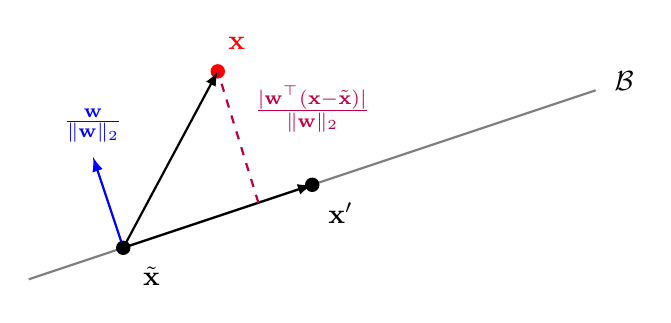
\begin{tikzpicture}[scale=1.2]
        % the decision boundary, with label
        \draw[gray, thick] (-3, -1) -- (3, 1);
        \node at (3.3, 1.1) {$ \mathcal{B} $};
        % w vector, with label (close to unit in length)
        \draw[blue, thick, -latex] (-2, -2/3) -- (-2.32, -2/3 + 0.96);
        \node[text=blue] at (-2.32, -2/3 + 1.29) {%
            $ \frac{\mathbf{w}}{\Vert\mathbf{w}\Vert_2} $%
        };
        % location of x prime, with label
        \filldraw[black] (0, 0) circle (2pt);
        \node at (0.3, -0.3) {$ \mathbf{x}' $};
        % location of x tilde, with label
        \filldraw[black] (-2, -2/3) circle (2pt);
        \node at (-1.7, -2/3 - 0.3) {$ \tilde{\mathbf{x}} $};
        % difference between x prime and x tilde
        \draw[black, thick, -latex] (-2, -2/3) -- (0, 0);
        % location of x, with label
        \filldraw[red] (-1, 1.2) circle (2pt);
        \node[text=red] at (-0.8, 1.5) {$ \mathbf{x} $};
        % difference between x and x tilde
        \draw[black, thick, -latex] (-2, -2/3) -- (-1, 1.2);
        % projection of x onto decision boundary, with label
        \draw[purple, thick, dashed] (-0.57, -0.19) -- (-1, 1.2);
        \node[text=purple] at (0, 0.8) {$ \frac{|\mathbf{w}^\top(\mathbf{x} -
        \tilde{\mathbf{x}})|}{\Vert\mathbf{w}\Vert_2} $};
    \end{tikzpicture}
    \caption{%
        An illustration of how $ |\mathbf{w}^\top(\mathbf{x} -
        \tilde{\mathbf{x}})| / \Vert\mathbf{w}\Vert_2 $ gives the distance
        of $ \mathbf{x} $ from $ \mathcal{B} $.%
    }
    \label{fig:3.2.1}
\end{figure}

% may or may not be needed depending on the page layout
%\medskip

Noting that $ yf(\mathbf{x}) > 0 $ if $ f $ classifies $ \mathbf{x} $
correctly, $ yf(\mathbf{x}) < 0 $ if $ f $ classifies $ \mathbf{x} $
incorrectly, and that $ f(\tilde{\mathbf{x}}) = 0 $, as
$ \tilde{\mathbf{x}} \in \mathcal{B} $, so we can manipulate the
$ \mathbf{w}^\top(\mathbf{x} - \tilde{\mathbf{x}}) / \Vert\mathbf{w}\Vert_2 $
expression to see that
\begin{equation*}
    y\frac{
        \mathbf{w}^\top(\mathbf{x} - \tilde{\mathbf{x}})
    }{
        \Vert\mathbf{w}\Vert_2
    } =
    y\frac{
        \mathbf{w}^\top(\mathbf{x} - \tilde{\mathbf{x}}) + b - b
    }{
        \Vert\mathbf{w}\Vert_2
    } =
    y\frac{f(\mathbf{x}) - f(\tilde{\mathbf{x}})}{\Vert\mathbf{w}\Vert_2} =
    \frac{yf(\mathbf{x})}{\Vert\mathbf{w}\Vert_2}
\end{equation*}

We thus indeed see that as stated, $ yf(\mathbf{x}) / \Vert\mathbf{w}\Vert_2 $
is the signed distance of $ \mathbf{x} $ from the decision boundary
$ \mathcal{B} $ defined by $ f $, where
$ yf(\mathbf{x}) / \Vert\mathbf{w}\Vert_2 $ is positive if $ f $ classifies
$ \mathbf{x} $ correctly and negative if $ f $ classifies $ \mathbf{x} $
incorrectly.

\newtocsubsection{Exercise 3.3}

Under the multinomial logistic regression model for $ K $ classes with $ d $
predictors, the softmax conditional likelihoods and therefore their logs are
invariant to constant shifts in the coefficient vectors
$ \mathbf{w}_1, \ldots \mathbf{w}_K \in \mathbb{R}^d $. More precisely, for
$ \mathbf{c} \in \mathbb{R}^d $, the conditional probabilities
$ \mathbb{P}_{\mathbf{W}, \mathbf{b}}\{Y = k \mid X = \mathbf{x}\} $ for each
class $ k $, where $ \mathbf{W} \triangleq \begin{bmatrix} \ \mathbf{w}_1 &
\ldots \mathbf{w}_K \ \end{bmatrix} \in \mathbb{R}^{d \times K} $ gives the
model coefficients and $ \mathbf{b} \in \mathbb{R}^K $ gives the intercepts,
are such that $ \mathbb{P}_{\mathbf{W}, \mathbf{b}}\{Y = k \mid
X = \mathbf{x}\} = \mathbb{P}_{\mathbf{W} - \mathbf{c}\mathbf{1}_K^\top,
\mathbf{b}}\{Y = k \mid X = \mathbf{x}\} $\footnote{
    Note that $ \mathbf{W} - \mathbf{c1}_K^\top = \begin{bmatrix}
        \ \mathbf{w}_1 - \mathbf{c} & \ldots & \mathbf{w}_K - \mathbf{c} \
    \end{bmatrix} $, so from (\ref{eq:logreg_softmax}) we see that
    \begin{equation*}
        \mathbb{P}_{\mathbf{W}, \mathbf{b}}\{
            Y = k \mid X = \mathbf{x}
        \} =
        \frac{e^{-\mathbf{c}^\top\mathbf{x}}}{e^{-\mathbf{c}^\top\mathbf{x}}}
        \left(
            \frac{
                e^{\mathbf{w}_k^\top\mathbf{x} + b_k}
            }{
                \sum_{k' = 1}^Ke^{\mathbf{w}_{k'}^\top\mathbf{x} + b_{k'}}
            }
        \right) =
        \frac{
            e^{(\mathbf{w}_k - \mathbf{c})^\top\mathbf{x} + b_k}
        }{
            \sum_{k' = 1}^K
            e^{(\mathbf{w}_{k'} - \mathbf{c})^\top\mathbf{x} + b_{k'}}
        } \triangleq
        \mathbb{P}_{\mathbf{W} - \mathbf{c1}_K^\top, \mathbf{b}}\{
            Y = k \mid X = \mathbf{x}
        \}
    \end{equation*}
}, where
\begin{equation} \label{eq:logreg_softmax}
    \mathbb{P}_{\mathbf{W}, \mathbf{b}}\{Y = k \mid X = \mathbf{x}\} \triangleq
    \frac{
        e^{\mathbf{w}_k^\top\mathbf{x} + b_k}
    }{
        \sum_{k' = 1}^Ke^{\mathbf{w}_{k'}^\top\mathbf{x} + b_{k'}}
    }
\end{equation}

However, the regularized part of the objective is not invariant to shifts and
can resolve the choice of $ \mathbf{c} $. In particular, for
$ \alpha \in [0, 1] $, using the elastic net penalty, we consider
\begin{equation} \label{eq:3.3.1}
    \min_\mathbf{c}\sum_{k = 1}^K\left[
        \frac{1}{2}(1 - \alpha)\Vert\mathbf{w}_k - \mathbf{c}\Vert_2^2 +
        \alpha\Vert\mathbf{w}_k - \mathbf{c}\Vert_1
    \right]
\end{equation}

Let $ \hat{\mathbf{c}}_\alpha $ solve (\ref{eq:3.3.1}) for a value of
$ \alpha $, $ \bar{\mathbf{w}} \triangleq \frac{1}{K}\mathbf{W1}_K =
\frac{1}{K}\sum_{k = 1}^K\mathbf{w}_k $, and let $ \tilde{\mathbf{w}} $ be the
median of $ \mathbf{w}_1, \ldots \mathbf{w}_K $. To make our analysis simpler,
first consider $ \hat{\mathbf{c}}_0 $, which is such that
\begin{equation} \label{eq:3.3.2}
    \hat{\mathbf{c}}_0 =
    \arg\min_\mathbf{c}\sum_{k = 1}^K
    \frac{1}{2}\Vert\mathbf{w}_k - \mathbf{c}\Vert_2^2
\end{equation}

(\ref{eq:3.3.2}) is easy to solve since it is differentiable. It is necessary
$ \mathbf{0} = \sum_{k = 1}^K(\mathbf{w}_k - \hat{\mathbf{c}}_0) =
\sum_{k = 1}^K\mathbf{w}_k - K\hat{\mathbf{c}}_0 $, so
\begin{equation} \label{eq:3.3.3}
    \hat{\mathbf{c}}_0 \triangleq
    \frac{1}{K}\sum_{k = 1}^K\mathbf{w}_k \triangleq \bar{\mathbf{w}}
\end{equation}

TODO

%Now we consider $ \hat{\mathbf{c}}_1 $, which is such that
%\begin{equation} \label{eq:3.3.4}
%    \hat{\mathbf{c}}_1 =
%    \arg\min_\mathbf{c}\sum_{k = 1}^K\Vert\mathbf{w}_k - \mathbf{c}\Vert_1
%\end{equation}

\section{Generalizations of the Lasso Penalty}

\newtocsubsection{Exercise 4.1}

Since the predictors are the same, let us consider a single predictor
$ X \triangleq X_1 = X_2 $. Therefore, the input matrix
$ \mathbf{X} \in \mathbb{R}^{N \times 2} $ can simply be written as
$ \mathbf{x1}^\top \in \mathbb{R}^{N \times 2} $, where
$ \mathbf{x} \in \mathbb{R}^N $ is a vector of realizations of $ X $. The
ridge regression in Lagrangian form for $ \lambda \in (0, \infty) $ is
therefore
\begin{equation} \label{eq:4.1.1}
    \begin{array}{rl}
        \displaystyle\min_{\mathbf{w}, b} &
        \frac{1}{2N}\left\Vert
            \mathbf{y} - \mathbf{x1}^\top\mathbf{w} - b\mathbf{1}
        \right\Vert_2^2 +
        \frac{1}{2}\lambda\Vert\mathbf{w}\Vert_2^2
    \end{array}
\end{equation}

As usual, let us make the usual standardization assumptions on $ \mathbf{x} $,
i.e. $ \frac{1}{N}\mathbf{1}^\top\mathbf{x} = 0 $,
$ \frac{1}{N}\mathbf{x}^\top\mathbf{x} = 1 $, so we know that the\footnote{
    It is easy to check that (\ref{eq:4.1.1}) is strictly convex in
    $ \mathbf{w} $, $ b $.
} optimal $ \hat{b} \triangleq \bar{y} $, where
$ \bar{y} \triangleq \frac{1}{N}\mathbf{1}^\top\mathbf{y} $. Therefore, at
the optimal $ \hat{\mathbf{w}} \in \mathbb{R}^2 $ we have
\begin{equation*}
    \mathbf{0} =
    -\frac{1}{N}\mathbf{1x}^\top\big(
        \mathbf{y} -  \mathbf{x1}^\top\hat{\mathbf{w}} - \bar{y}\mathbf{1}
    \big) +
    \lambda\hat{\mathbf{w}} =
    -\frac{1}{N}\mathbf{1x}^\top\mathbf{y} +
    \left(\mathbf{11}^\top + \lambda\mathbf{I}\right)\hat{\mathbf{w}}
\end{equation*}

It is easy to verify that $ \forall c, d \in (0, \infty) $,
$ c\mathbf{11}^\top + d\mathbf{I} \succ \mathbf{0} $, and so we can rearrange
the above to see that
\begin{equation} \label{eq:4.1.2}
    \hat{\mathbf{w}} =
    \frac{1}{N}\left(
        \mathbf{11}^\top + \lambda\mathbf{I}
    \right)^{-1}
    \mathbf{1x}^\top\mathbf{y}
\end{equation}

(\ref{eq:4.1.2}) holds in general for any $ \mathbf{X} \in \mathbb{R}^d $ that
duplicates the same column $ d $ times, but since
$ \hat{\mathbf{w}} \in \mathbb{R}^2 $, we can invert
$ \mathbf{11}^\top + \lambda\mathbf{I} $ by hand to get explicit expressions
for $ \hat{w}_1 $, $ \hat{w}_2 $. We see that
\begin{equation} \label{eq:4.1.3}
    \left(\mathbf{11}^\top + \lambda\mathbf{I}\right)^{-1} \triangleq
    \begin{bmatrix}
        \ 1 + \lambda & 1 \ \\ \ 1 & 1 + \lambda \
    \end{bmatrix}^{-1} =
    \frac{1}{(1 + \lambda)^2 - 1}
    \begin{bmatrix}
        \ 1 + \lambda & -1 \ \\ \ -1 & 1 + \lambda \
    \end{bmatrix} =
    \frac{1}{2\lambda + \lambda^2}
    \begin{bmatrix}
        \ 1 + \lambda & -1 \ \\ \ -1 & 1 + \lambda \
    \end{bmatrix}
\end{equation}

From (\ref{eq:4.1.3}), we see that $ \left(\mathbf{11}^\top +
\lambda\mathbf{I}\right)^{-1}\mathbf{1} = \frac{1}{2 + \lambda}\mathbf{1} $,
so we can define $ \hat{w} \triangleq \hat{w}_1 = \hat{w}_2 $, i.e.
$ \hat{\mathbf{w}} = \hat{w}\mathbf{1} $, where
\begin{equation} \label{eq:4.1.4}
    \hat{w} =
    \frac{1}{N}\left(\frac{\mathbf{x}^\top\mathbf{y}}{2 + \lambda}\right)
\end{equation}

(\ref{eq:4.1.4}) shows that $ \hat{w}_1 $, $ \hat{w}_2 $ are identical,
directly proportional to $ \frac{1}{N}\mathbf{x}^\top\mathbf{y} $, and
inversely proportional to $ \lambda $.

\section{Optimization Methods}

\newtocsubsection{Exercise 5.1}

We consider the function $ f : \mathbb{R}^d \rightarrow \mathbb{R} $, where
for $ \mathbf{b} \in \mathbb{R}^d $, $ \mathbf{Q} \succ \mathbf{0} \in
\mathbb{R}^{d \times d} $,
\begin{equation} \label{eq:5.1.1}
    f(\mathbf{x}) \triangleq
    \frac{1}{2}\mathbf{x}^\top\mathbf{Qx} - \mathbf{b}^\top\mathbf{x}
\end{equation}

\begin{enumerate}[label=\alph*.]
    \item
    Since $ \mathbf{Q} \succ \mathbf{0} $ and from inspection $ f $ is twice
    differentiable, with $ \nabla^2f(\mathbf{x}) = \mathbf{Q} $,
    $ \forall \mathbf{x} \in \mathbb{R}^d $, $ f $ is strictly convex. We can
    verify the uniqueness of its minimizer $ \mathbf{x}^* $ as $ f $ strictly
    convex $\Leftrightarrow \forall \mathbf{x}, \mathbf{x}' \in
    \mathbb{R}^d $, $ \mathbf{x} \ne \mathbf{x}' $,
    \begin{equation} \label{eq:5.1.2}
        f(\mathbf{x}') >
        f(\mathbf{x}) + \nabla f(\mathbf{x})^\top(\mathbf{x}' - \mathbf{x})
    \end{equation}
    Since necessarily $ \nabla f(\mathbf{x}^*) = \mathbf{0} $,
    $ \forall \mathbf{x} \in \mathbb{R}^d $, $ \mathbf{x} \ne \mathbf{x}^* $,
    from (\ref{eq:5.1.2}) we have $ f(\mathbf{x}) > f(\mathbf{x}^*) $.
    Furthermore, since $ \nabla f(\mathbf{x}^*) = \mathbf{Qx}^* - \mathbf{b} =
    \mathbf{0} $ and $ \mathbf{Q} \succ \mathbf{0} \Rightarrow \mathbf{Q} $
    invertible, then
    \begin{equation} \label{eq:5.1.3}
        \mathbf{x}^* = \mathbf{Q}^{-1}\mathbf{b}
    \end{equation}

    \item
    Letting $ \eta \in (0, \infty) $ be the step size, for a sequence of
    $ \{\mathbf{x}_n\}_{n \in \mathbb{N}} $ of approximations to
    $ \mathbf{x}^* $ yielded by gradient descent from an initial guess
    $ \mathbf{x}_0 $, the $ n $th term $ \mathbf{x}_n $ is such that
    \begin{equation} \label{eq:5.1.4}
        \mathbf{x}_n =
        \mathbf{x}_{n - 1} - \eta(\mathbf{Qx}_{n - 1} - \mathbf{b})
    \end{equation}

    \item
    First, we write (\ref{eq:5.1.4}) more conveniently such that
    $ \mathbf{x}_{n - 1} $ only occurs once, as
    \begin{equation} \label{eq:5.1.5}
        \mathbf{x}_n =
        (\mathbf{I} - \eta\mathbf{Q})\mathbf{x}_{n - 1} + \eta\mathbf{b}
    \end{equation}

    TODO
\end{enumerate}

\end{document}